\addcontentsline{toc}{chapter}{An Introduction to Tracking Loops}\label{ch:TrackingLoops}
\chapter{An Introduction to Tracking Loops}
In summary, the goal of the carrier tracking loop is to predict the future carrier phase $\phi$,$T$ seconds in the future, based on past and current measurements of the carrier phase. For successful phase lock to be maintained, the predicted phase must be within a small fraction of a cycle of the actual phase. 

\section{Ambiguities}

We can describe the elapsed phase (in radians) between the satellite and the receiver using the following equation :  
\begin{equation}
Phase = 2 \pi N  + \phi 
\label{eq:Phase}
\end{equation}

If we examine equation \ref{eq:Phase} in the spatial domain, we find that: 
\begin{equation}
Range = \lambda N + \Phi
\label{eq:Distance}
\end{equation}

From Equations \ref{eq:Phase} and \ref{eq:Distance} it is obvious that prediction of the angular phase $\phi$ is equivalent to prediction of the spatial phase $\Phi$.

It is important to note, that predicting $\Phi$ is equivalent to predicting the change in the LOS range ($\Delta$), hence the receiver does not need to be aware of the number of full cycles $N$, between it and the satellite. This ambiguity is the one that is resolved during the process of carrier phase positioning. 

\section{Error bounds}
In the case of the GPS signal, where the $L_1$ 1.575Ghz signal is being tracked, the carrier wavelength, $\lambda \approx 19.03 cm$ long. As a heuristic, the difference between the actual carrier phase $\phi$ , and the predicted carrier phase $\hat{\phi}$ must be no more than $\pm30 \degree$. 

This concept is clearly illustrated in figure \ref{fig:PhaseDelay}. 

Denoting our prediction of $\Delta$ as $\hat{\Delta}$, we have :

\begin{align}
|\Delta-\hat{\Delta}|& < \frac{30\degree}{360\degree} \lambda\\
|\Delta-\hat{\Delta}|&<\epsilon\\
|\Delta-\hat{\Delta}|&<1.58cm\\
\label{eq:RangeErrorBound}
\end{align}

Hence, our estimate of $\Delta$ must be accurate to $< 1.58cm$, if the receiver is to remain in phase lock.

By examining figure \ref{fig:ValidPositions} we can begin to understand that the locus of all possible positions which meet this criteria is a spherical shell surrounding the satellite. 

When we consider that GPS utilises multiple satellites for positioning, we can conclude with the aid of figure \ref{fig:Intersections} that a bound on the magnitude of the error is formed by the sphere of radius $\epsilon$ surrounding the point X, which is the true position of the receiver. 

Hence, we have :

\begin{comment}
\begin{align}
| X(t)-\hat{X}(t) | & < \frac{30\degree}{360\degree} \lambda \\
| X(t)-\hat{X}(t) | &<\Delta\\
| X(t)-\hat{X}(t) | & < 1.58cm
\label{eq:PositionErrorBound}
\end{align}
\end{comment}

\section{Mechanics}

By conceptualising we can immediately gain insight into some of the fundamental challenges that will be faced in the development of tracking algorithms for coping with high dynamics.

\tikzset{
block/.style = {draw, fill=white, rectangle, minimum height=3em, minimum width=3em},
tmp/.style  = {coordinate}, 
sum/.style= {draw, fill=white, circle, node distance=1cm},
input/.style = {coordinate},
output/.style= {coordinate},
pinstyle/.style = {pin edge={to-,thin,black}
}
}

\begin{figure}[!htb]
\centering

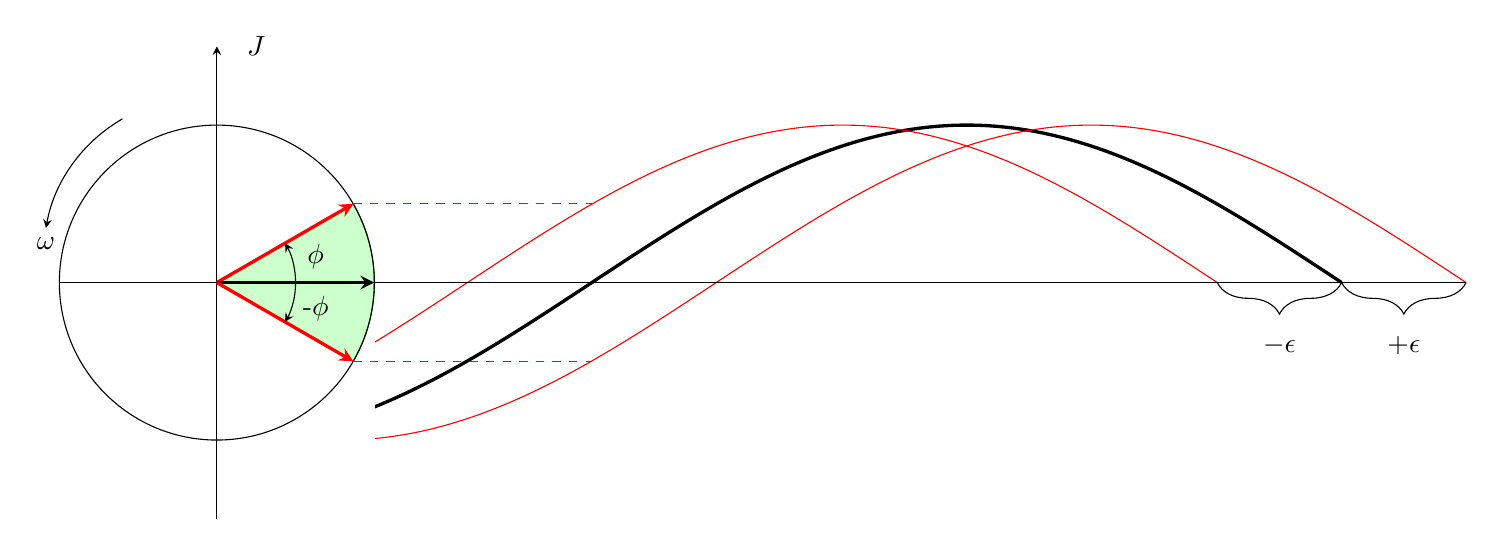
\begin{tikzpicture}
    
    \draw[black,very thick] (0,-2) cos (4.76175,0) sin (2*4.76175,2) cos (3*4.76175,0) ;
    
    \draw[red] (-1.58,-2) cos (4.76175-1.58,0) sin (2*4.76175-1.58,2) cos (3*4.76175-1.58,0) ;
    
    \draw[red] (1.58,-2) cos (4.76175+1.58,0) sin (2*4.76175+1.58,2) cos (3*4.76175+1.58,0) ;
    
    \draw [decorate,decoration={brace,amplitude=0.4cm},xshift=0,yshift=0pt]
(3*4.76175+1.58,0) -- (3*4.76175,0) node [black,midway]{};
    \node at (3*4.76175+0.5*1.58,-0.8) {$+\epsilon$};
    
    \draw [decorate,decoration={brace,amplitude=0.4cm,mirror},xshift=0,yshift=0pt]
(3*4.76175-1.58,0) -- (3*4.76175,0) node [black,midway]{};
    \node at (3*4.76175-0.5*1.58,-0.8) {$-\epsilon$};

    \draw [fill opacity=1, fill=white,white] (-1.58,0.1) rectangle(2,-2.1);
    
    \filldraw[fill=green!20!white, draw=green!50!black]
    (0,0) -- (-30:2) arc (-30:30:2) -- cycle;
    \draw (0,0) circle (2cm);
    
    \draw[->,-stealth,color=black] (0,-3) -- (0,3);
    \node at (0.5,3) {$J$};
    
    \draw(-2,0) -- (3*4.76175+1.58,0);
    
    \draw[->,color=red, very thick,-stealth] (0,0)--(30:2);
    \draw[->,color=black, very thick,-stealth ] (0,0)--(0:2);
    \draw[->,color=red, very thick,-stealth ] (0,0)--(-30:2);
    
    \draw[-,color=red, dashed] (30:2)--(4.76175,1);
    \draw[-,color=red, dashed] (-30:2)--(4.76175,-1);
    
    \draw[->,-stealth ]  (0:1cm) arc (0:30:1cm);
    \draw[->,-stealth ]  (0:1cm) arc (0:-30:1cm);
    
    \node at (15:1.3) {$\phi$};
    \node at (-15:1.3) {-$\phi$};
    % angular velocity \omega
    \draw[->,-stealth ]  (120:2.4cm) arc (120:170:2) node[below] {$\omega$};
    
    \end{tikzpicture}
\caption{A scale drawing of the tolerances required for successful phase lock of the GPS $L_1$ signal.The phase, $\phi$ of the locally generated carrier (red) needs to remain within $30\degree$ of the phase the incoming carrier (black). This equates to a $\Delta$ range of 1.58 cm to the satellite.} \label{fig:PhaseDelay}
\end{figure}


\tikzset{
block/.style = {draw, fill=white, rectangle, minimum height=3em, minimum width=3em},
tmp/.style  = {coordinate}, 
sum/.style= {draw, fill=white, circle, node distance=1cm},
input/.style = {coordinate},
output/.style= {coordinate},
pinstyle/.style = {pin edge={to-,thin,black}
}
}

\begin{figure}[!htb]
\centering

\begin{tikzpicture}
    \newcommand\Radius{6} 
    \filldraw[fill=green!20!white, draw=green!50!black]
    (0:\Radius+1.58) arc (0:360:\Radius+1.58) -- cycle;
    
    \filldraw[fill=white, draw=green!50!black]
    (0:\Radius-1.58) arc (0:360:\Radius-1.58) -- cycle;
    
    \draw[draw=green!50!black,dashed]
    (0:\Radius) arc (0:360:\Radius) -- cycle;
    
    \draw[->,color=black,-stealth, thick] (0,0)--(30:\Radius+1.58);
    \draw[->,color=black,-stealth, thick] (0,0)--(90:\Radius);
    \draw[->,color=black,-stealth, thick] (0,0)--(150:\Radius-1.58);
    
    
    \node at (20:3) {$r+\Delta$};
    \node at (95:3) {$r$};
    \node at (160:3) {$r-\Delta$};
    \node at (0,-0.25) {Satellite};
    
    \end{tikzpicture}
\caption{In order to maintain phase lock with a single satellite, the predicted range to the satellite used to generate the phase, must lie inside an spherical shell, centred around the true range to the satellite. The shell is visualised as an annulus which is bounded by $r-\epsilon<r<r+\epsilon$. $\epsilon$ is depicted at 1:1 scale.} \label{fig:ValidPositions}
\end{figure}


\tikzset{
block/.style = {draw, fill=white, rectangle, minimum height=3em, minimum width=3em},
tmp/.style  = {coordinate}, 
sum/.style= {draw, fill=white, circle, node distance=1cm},
input/.style = {coordinate},
output/.style= {coordinate},
pinstyle/.style = {pin edge={to-,thin,black}
}
}

\begin{figure}[!htb]
\centering

\begin{tikzpicture}
    %\filldraw[fill=green!20!white, draw=green!20!white]
    %(-59.5:7.58) arc (-59.5:-120.5:7.58) arc (147:32:4.58) %--cycle;
    
    \filldraw[fill=green!20!white, draw=green!20!white]
    (-46:5.58) arc (-46:-134:5.58) arc (134.5:46:5.58);
    
    
    \newcommand\RadiusA{4} 
    \draw[draw=black]
    (0:\RadiusA+1.58) arc (0:360:\RadiusA+1.58) -- cycle;
    
    \draw[draw=black]
    (0:\RadiusA-1.58) arc (0:360:\RadiusA-1.58) -- cycle;
    
    \draw[draw=black,dashed]
    (0:\RadiusA) arc (0:360:\RadiusA) -- cycle;
    
    \node at (0,0) {Satellite A};
    
    \newcommand\RadiusB{4} 
    \draw[draw=black]
    (\RadiusB+1.58,-8) arc (0:360:\RadiusB+1.58) -- cycle;
    
    \draw[draw=black]
    (\RadiusB-1.58,-8) arc (0:360:\RadiusB-1.58) -- cycle;
    
    \draw[dashed]
    (\RadiusB,-8) arc (0:360:\RadiusB) -- cycle;
    
    \node at (0,-8) {Satellite B};
    
    \node at (0,-4.35) {$X$};
    
    \end{tikzpicture}
\caption{In the case of multiple satellites, the only viable positions where phase lock can be maintained is the union between the spherical shells of the satellites, visualised here as annuli. As the number of different satellites increases, the bounding volume of the solution approaches a sphere with radius 2 $\epsilon$ centred at the true position X. $\epsilon$ is depicted at 1:1 scale.}
\label{fig:Intersections}
\end{figure}



Returning to first principles of mechanics, we have \cite{salas1999etgen} : 

\begin{comment}
Need to fix this up
\end{comment}

\begin{align}
v & = \frac{\Delta}{T} m s^{-1} \\
a & = \frac{dv}{dt} m s^{-2} \\
Jerk & = \frac{da}{dt} m s^{-3}
\end{align}


Note that over time, the acceleration of the receiver is integrated to form it's velocity, and the velocity is integrated in order to form it's position. 

Note that our estimate of the position $\hat{X}(t+T)$ is dependent on our current velocity $\dot{X}(t)$. When use this velocity, we are implicit assuming that the average velocity for the next time period is the same. 

However,as illustrated in figure \ref{fig:PhaseDelay}, and in equation \ref{eq:RangeErrorBound}, our estimate of the new range to the satellite must fall within 
position must fall within a close 

our estimate of the velocity must fall within the following bounds:



\begin{equation}
V_{min} < \hat{\dot{X}}(t) < V_{max}
\end{equation}





\section{Motion models}

Given we are attempting to predict the carrier $T$ seconds into the future, we can start to investigate the maximum dynamics our receiver will be able to track for a given sampling period $T$. \cite{salas1999etgen}


\begin{equation}
X = \int_{t_1}^{t_2} \dot{X} dt + X(t_1)
\label{eq:PositionIntergral}
\end{equation}

\begin{equation}
\dot{X} = \int_{t_1}^{t_2} \ddot{X} dt + \dot{X}(t_1)
\end{equation}


Equation \ref{eq:PositionIntergral} suggests that we can form an prediction of the range to the satellite using the current range and the current line of sight velocity. 

\begin{equation}
\hat{X}(t+T) = X(t) +  \dot{X}(t) T
\end{equation}

\begin{equation}
t = nT
\end{equation}

\begin{equation}
\hat{X}[n+1] = X[n] +  \dot{X}[n] T
\end{equation}






Equation 5.7
\begin{equation}
\sigma_{PLLt} = \frac{\lambda_L}{2 \pi} \sqrt{\frac{B_n}{C/N_0}(1+\frac{1}{2 \cdot T \cdot C/N_0})} \text{ (m)}
\end{equation}
%\cite{Kaplan}

Where:
\begin{align*}
B_n &= \text{carrier loop noise bandwidth (Hz)} \\
C/N_0 &= \text{carrier to noise power ratio in (Hz)} \\
&=10^\frac{(C/N_0)_dB}{10} \\
T &= \text{pre-detection (coherent) integration time (s)} \\
\lambda_L &= \text{GPS L1 carrier wavelength (m)}\\
&= 0.1903 m
\end{align*}

%\cite{Kaplan} \cite{Jwo}




\begin{comment}
This document provides and overview of the Namuru carrier tracking loop architecture. The software architecture has evolved over time, and uses elements of different approaches from the literature, as well as a number of novel components implemented by Dr Eamonn Glennon. 

\section{Current Namuru architecture}

The Namuru receiver currently uses a third-order PLL loop filter with a second-order FLL assist. This architecture can be seen in figure .  A third order PLL uses a second order filter, with the third integrator being the VCO.

Namuru additionally has a code tracking loop, however will not be discussed in this document. The dynamics experienced by the code tracking loop are 1540 times smaller than those experienced by the carrier loop \cite{Kaplan}. Hence the  code loop is significantly more robust than either the FLL or PLL.

The PLL is the most vulnerable of the loops, and under extreme dynamics, the PLL will break and the FLL will keep tracking, before the PLL resumes tracking once the dynamics have subsided to more reasonable levels. Hence, while the FLL is described, more effort will be expended on analysis of the PLL.

\section{Tracking Loops}

The receiver implements a digital (sampled) phase lock loop (PLL), the theoretical background of which is covered thoroughly in Gardner \cite{Gardner}. 
 
Additionally, the receiver also implements a FLL, which is used to assist the PLL in locking.

Both of the loops include a number of components that will be discussed in more detail later, 

\begin{itemize}
\item{Discriminator}
\item{Integrate \& Dump}
\item{Loop Controller/Loop Filter}
\item{Hold}
\item{Delay}
\item{NCO}
\end{itemize}

In the they key difference between the two filters is the discriminator. 
\end{comment}